\subsection{Gui-Quellpaket}
    \subsubsection{ScotlandYard}
        \begin{table}[H]
            \caption{Klasse ScotlandYard}
            \begin{tabular}{p{2.5cm}  p{9.5cm}} 
                \hline
                \textbf{Eigenschaft} & \textbf{Beschreibung}\\
                \hline
                Name & ScotlandYard\\
                Ort & Source-Paket \textit{gui}\\
                \hline
                Zweck &
                Enthält die \textit{main}-Methode die eine JavaFX-Applikation startet.\\
                \hline
                Beschreibung &
                \begin{itemize}
                    \itemsep0em
                    \item Lädt die FXML-Datei und baut die \textit{Stage} und die \textit{Scene} auf
                    \item Übergibt die Kontrolle an den \textit{FXMLController}
                \end{itemize}
                \\
                \hline
            \end{tabular}
        \end{table}
        \begin{figure}[H]
            \centering
            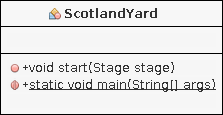
\includegraphics[scale=0.7]{img/uml/scotlandYard.png}   
            \caption{ScotlandYard UML-Klassendiagramm}
        \end{figure}


    \subsubsection{FXMLDocumentController}
        \begin{table}[H]
            \caption{Klasse FXMLDocumentController}
            \begin{tabular}{p{2.5cm}  p{9.5cm}} 
                \hline
                \textbf{Eigenschaft} & \textbf{Beschreibung}\\
                \hline
                Name & FXMLDocumentController\\
                Ort & Source-Paket \textit{gui}\\
                \hline
                Zweck &
                Wird beim Programmstart geladen. Die Klasse kennt alle Element aus der FXML-Datei.
                Führt für Interaktionen mit der GUI die entsprechenden Handler aus.
                \\
                \hline
                Beschreibung &
                \begin{itemize}
                    \itemsep0em
                    \item Instanziiert eine \textit{JavaFXGui}-Instanz und übergibt dieser alle benötigten FXML-Elemente
                    \item Instanziiert eine \textit{GameLogic}-Instanz und übergibt dieser die \textit{JavaFXGui}-Instanz
                    \item Reicht alle Interaktionen von der GUI weiter an die \textit{GameLogic} damit sie dort verarbeitet werden können
                \end{itemize}
                \\
                \hline
            \end{tabular}
        \end{table}
        \begin{figure}[H]
            \centering
            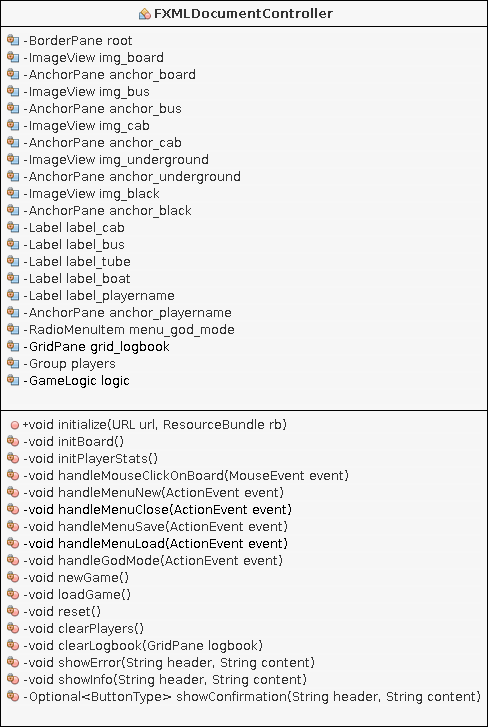
\includegraphics[scale=0.65]{img/uml/fxmlDocumentController.png}   
            \caption{FXMLDocumentController UML-Klassendiagramm}
        \end{figure}


    \subsubsection{FXMLDocument.fxml}
        Die Datei enthält alle graphischen Elemente die für das \textit{ScotlandYard} benötigt werden.
        Darunter zählen \textit{Id}'s oder auch Methoden die eine Interaktion erlauben.
        Diese Datei wird benötigt um die GUI aufzubauen und mit ihr zu interagieren.

    \subsubsection{JavaFXGui}
        \begin{table}[H]
            \caption{Klasse JavaFXGui}
            \begin{tabular}{p{2.5cm}  p{9.5cm}} 
                \hline
                \textbf{Eigenschaft} & \textbf{Beschreibung}\\
                \hline
                Name & JavaFXGui\\
                Ort & Source-Paket \textit{gui}\\
                \hline
                Zweck &
                Implementiert, das von der \textit{Logic} vorgeschriebene \textit{GUIConnector-Interface}.
                Dadurch kann die \textit{GameLogic} auf Elemente der graphischen Oberfläche zugreifen.
                \\
                \hline
                Beschreibung &
                \begin{itemize}
                    \itemsep0em
                    \item Erhält beim Instanziieren alle nötigen Elemente der graphischen Oberfläche
                    \item Implementiert Methoden zur Darstellung der Spieler und ihrer Informationen
                    \item Implementiert Methoden zur Darstellung von Dialogen und sowie Infomeldungen
                \end{itemize}
                \\
                \hline
            \end{tabular}
        \end{table}
        \begin{figure}[H]
            \centering
            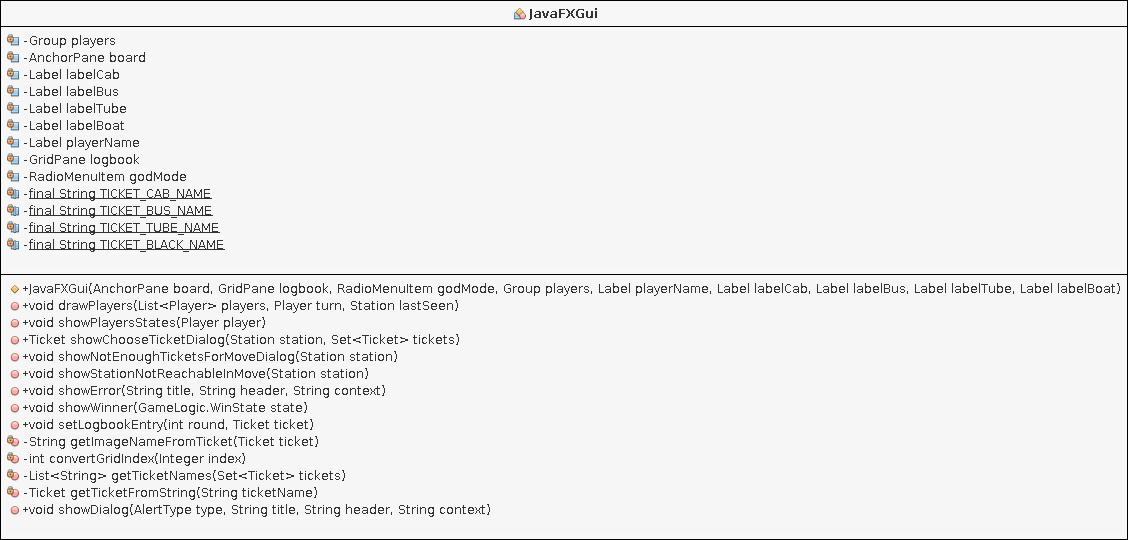
\includegraphics[scale=0.35]{img/uml/javaFXGui.png}   
            \caption{JavaFXGui UML-Klassendiagramm}
        \end{figure}


